\chapter{Methodology}
\section{Spectrum Sensing} \label{methods:processing}
The main goal of this system is to be able to detect wireless signals. In order to do so, the following sensing methods were used.
\subsection{Energy Detection}
The system detects transmissions based off of energy detection. This type of detection is done by measuring our received signal’s strength along a desired central frequency, and comparing it to an ideal threshold. In order to determine the energy of the received signal, the following equation was used:
\[E = \int_{-\infty}^{\infty}| x(t) |^2dt\]
This energy measurement is then compared to a threshold energy of -85 dBm. This threshold was chosen due to it being high enough to ensure a low chance of false alarm while still sensing signals from a significant distance, which is necessary since the drone will be high in the air. \par

In order to categorize WiFi signals at the 2.4GHz band, an OFDM detector was implemented. In order to detect OFDM, the receiver will detect beacon frames by correlating upon the WiFi’s L-STF structure. The L-STF structure is a specific spacing and timing of transmissions over various subcarriers. This structure is also used for calculating the coarse frequency offset. The subcarriers and transmissions used in L-STF are shown in Figure \ref{fig:ofdm_subcarriers}. \par 
\begin{figure}[ht!]
	\centering
	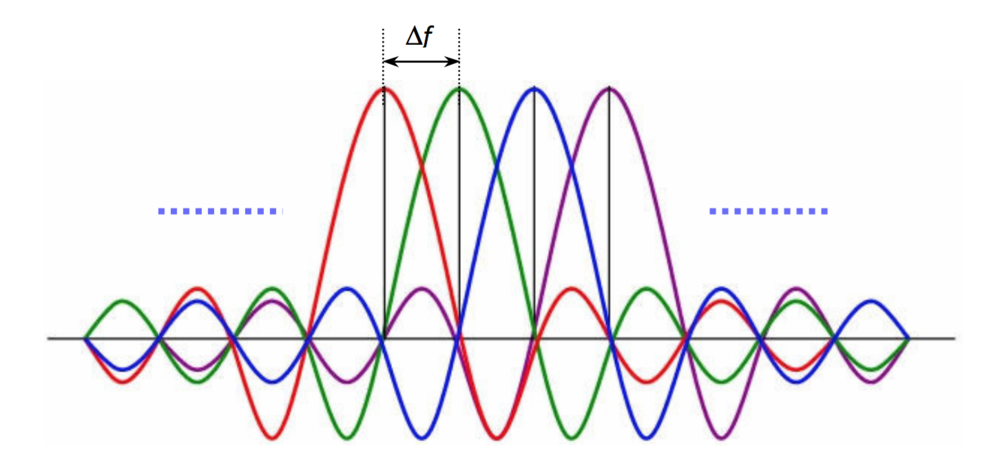
\includegraphics[width=0.70\textwidth]{img/ofdm-subcarriers}
	\caption{OFDM Subcarriers}
	\label{fig:ofdm_subcarriers}
\end{figure}\par
%(https://static1.squarespace.com/static/54860cc3e4b020d690f237ba/t/556cc531e4b0a02f64b72fed/1433191737073/ofdm-subcarriers?format=1000w)
The multiple subcarriers are represented by the various waveform colors in Figure \ref{fig:ofdm_subcarriers}. The spacing of each frequency is denoted by f. This series of waveforms are transmitted from the OFDM transmitter over a fixed amount of time. The spacing and frequency behavior of the L-STF field has the following characteristics: \par
\begin{table}[ht!]
	\centering
\begin{tabular}{|p{3.6cm}|p{4cm}|p{4cm}|p{4.5cm}|}
	\hline
	Channel Bandwidth\newline(MHz) & Subcarrier Frequency Spacing, $\Delta_F$ (kHz) &Fast Fourier Transform Period\newline($T_{FFT}=1/\Delta_F$)& L-STF duration \newline($T_{SHORT}=10*T_{FFT}/4$) \\
	\hline
	20,40,80,160 & 312.5 &3.2$\mu s$ &8 $\mu s$ \\
	10 & 156.25 &$6.4\mu s$ &16 $\mu s $\\
	5 & 78.125 &$12.8\mu s$ &32 $\mu s$  \\
	\hline
\end{tabular} 
	\caption{L-STF Characteristics}
	\label{table:spacing}
\end{table} \par 
	
Once a beacon transmission is detected using the above techniques, the L-SIG field must be decoded in order to determine the modulation, MCS rate, and length of the transmission.
\begin{figure}[ht!]
	\centering
	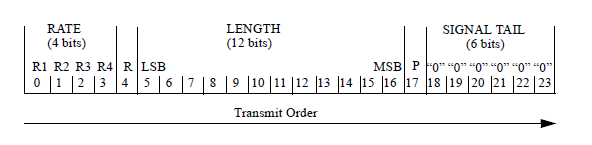
\includegraphics[width=0.70\textwidth]{img/lsig_packet}
	\caption{L-SIG Packet}
	\label{fig:lsig_packet}
\end{figure}\par
 The data frame for the L-SIG field is detailed in Figure \ref{fig:lsig_packet}.
\begin{table}[ht!]
	\centering
	\begin{tabular}{|c|c|c|c|}
		\hline
		802.11 version & Transmission Vector Format & Modulation Format & Bandiwdths(MHz) \\
		\hline
		802.11b & non-HT & DSSS/CCK  & 11 \\
		802.11a & non-HT & OFDM only & 5,10,20 \\
		802.11j & non-HT & OFDM only & 10 \\
		802.11p & non-HT & OFDM only & 5,10 \\
		802.11g & non-HT & OFDM      & 20 \\
			    & non-HT & DSSS/CCK  & 11 \\
		802.11n & HT\_MF,non-HT & OFDM only & 20,40 \\
		802.11ac & VHT,HT\_MF,non-HT & OFDM only & 20,40,80,160 \\
		802.11ah & s1G & OFDM only & 1,2,4,8,16 \\
		\hline
	\end{tabular}
	\caption{Details about Various WiFi transmission techniques}
	\label{table:WiFi_table}
\end{table} \par
The rate field gives us information such as the modulation, coding rate, and data rate by relating the rate to its respective binary value:

\begin{table}[ht!]
	\centering
	\begin{tabular}{|l|l|l|l|l|}
		\hline
		Rate(bits 0-3) & Modulation & Coding Rate (R) & 20 MHz data rate (Mb/s)\\
		1101 & Modulation & BPSK & 1/2 & 6 \\
		1111 & Modulation & BPSK & 3/4 & 9 \\
		0101 & Modulation & QPSK & 1/2 & 12 \\
		0111 & Modulation & QPSK & 3/4 & 18 \\
		1001 & Modulation & 16-QAM & 1/2 & 24 \\
		1011 & Modulation & 16-QAM & 3/4 & 36 \\
		0001 & Modulation & 64-QAM & 2/3 & 48 \\
		0011 & Modulation & 64-QAM & 3/4 & 54 \\						
		\hline
	\end{tabular}
	\caption{This table gives the corresponding modulation, coding rate, and data rate based on the received binary information from the L-STG field. These fields can then be used to further demodulate the received signal.}
	\label{table:ofdm_rate_table}
\end{table} \par

\begin{figure}[ht!]
	\centering
	
\includegraphics[width=0.70\textwidth]{img/filler}
	\caption{Rate Field Table \textbf{WE GONNA NEED THIS TO NOT BE FILLER}}
	\label{fig:ofdm_rate_table}
\end{figure}\par
Using the rate information, the received packet's 802.11 frame can be further analyzed to find the broadcast SSID of our received transmission frame. The SSID field which starts at the 36th byte of the beacon frame header is the only desired information here as it allows the identification of separate access points.
\begin{figure}[ht!]
	\centering
	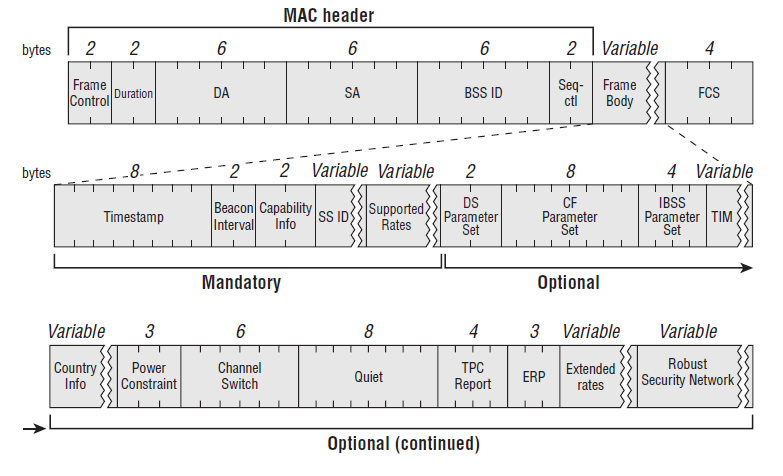
\includegraphics[width=0.70\textwidth]{img/beacon_frame}
	\caption{Beacon Frame Structure}
	\label{fig:beacon_frame}
\end{figure}\par
By converting these bits to ASCII, the SSID of the received transmission will be obtained.
\subsection{Signal Detection Summary}
Using a combination of energy detection and match filtering on OFDM beacon frames, the MASDR system will be able to identify the desired signals with a high probability of detection and a low probability of false alarm. Additionally, this will allow accurate determination of the received SSID.

\section{Fusion and Localization}
In order to draw meaning from the spectrum being measured, two types of data need to be analyzed: received signal strength (RSS) and location. Both of these measurements have noise to some extent. In this section, the combination of these measurements and the mitigation of sensor noise will be discussed. \par  

\subsection{RSS and Direction Readings}
After identifying a signal, the next step is to locate the signal source. Out of the methods described in the background, most are ruled out based on the non-cooperative nature of the sensing, leaving only Angle of Arrival (AoA) and RSS localization. Of those two methods, Angle of Arrival is the significantly more complex method to implement, requiring either a strongly directional antenna or an array of antennas \cite{local_aoa}. As such, RSS localization was the method implemented. This method requires three stationary observation points, as opposed to the single moving observation point contained on the aerial platform. To get around this requirement, it is assumed that the device broadcasting the WiFi is stationary \cite{rss_calc}. This assumption is valid because most access points are indeed stationary and the drone moves quickly enough that even a slowly moving signal would likely be able to be roughly located. \par 
Occasionally while sampling, the drone will rotate continuously in a process described in Implementation Section \ref{impl:rotate}. This presents a complication to the processing of the signal: only one sample is recorded at a given angle. Because the samples must be processed in blocks, each block will represent samples from a range of angles. Since the heading measurement is not implemented in the current version of the system, this is of little concern, but for future use, the scenario has been analyzed. \par
The angles included in a block are determined by the amount the drone rotates between the first sample and the last sample of the block. In a small enough block, the error generated by the difference in direction is minimal. However, a smaller block represents a smaller amount of time, in which the signal is more prone to being affected by noise. One solution is to slow down the angular velocity of the drone. While this can be done, the resulting design would be less modular, depending more heavily on the programmability of the drone in use. The other solution is to increase the block size, increasing the amount of time measured, but introducing the problem of deciding what direction should correspond with the resulting signal measurement. Regardless of how this is chosen, the larger block size increases the error in the localization measurement.\par 
%\begin{figure}[ht!]
%	\centering
%	\includegraphics[width=0.70\textwidth]{img/solo_measure}
%	\caption{L-SIG Packet}
%	\label{fig:solo_measure}
%\end{figure}\par
In a magnetometer enabled version of the system, a block size of 131,072 should be chosen. The 3DR Solo rotates at around 2 seconds per rotation. This means that it takes roughly 0.0222 seconds to rotate 4 degrees. At a sample rate of 5 MSPS, this is 111,111 samples. In order to input the signal into the FFT, the block size has to be a power of 2. The nearest power of 2 is $2^{17}$, which is 131072. Each block consists of the second half of the previous block and the next half block of samples. The first block has no previous block, so is just the first 16384 samples. The processed measurement is associated with the direction in the middle of the angle sweep covered by the block. This method introduces a maximum of one degree of error, which is on the same order of magnitude as the error in the HMC5883L magnetometer, a common chip \cite{magnetometer_data}. \par 
The shifting nature of wireless channels introduces a difficult to predict noise into the measurements taken. In order to mitigate this, the drone can rotate multiple times. The resulting received signal strength measurements can then be averaged with the readings from each rotation. This averaging reduces the chance that a random shift in the channel will negatively impact the direction readings. \par 
\subsection{GPS}
The MASDR system uses GPS readings for location. The distance of the beacon from the drone at multiple points is then used to get an estimated location of the beacon. Within a GPS receiver, signal correction is already being carried out. This results in a cleaner and usually more accurate measurement. In addition to this, the receiver that is used in this project polls much less frequently than the localization technique, at around 10 times a second. Since this is higher frequency than is needed, the readings are put through a Kalman Filter to increase the location accuracy. \par 
\subsection{Kalman Filtering}\label{methods:kf}
The GPS receiver that is used in this project provides very noisy results. A contributing factor to this is that the receiver used is both small and cheap. Because of this, the values that it reads are frequently very scattered, with a high variance. In order to mitigate this, a four-state Kalman Filter was designed and simulated in MATLAB. The Kalman Filter equations presented in the Background section are reproduced below \cite{kf_book}: \par
\subsubsection*{Predict:}
\begin{align}
    \vec{x} &= \matr{F}\vec{x} + \matr{H}\vec{u} \label{eq:state_predict}\\ 
    \matr{P} &= \matr{F}\matr{P}\matr{F^T} + \matr{Q} \label{eq:var_predict}
\end{align}
\subsubsection*{Update:}
\begin{align}
    \vec{y} &= \vec{M} - \matr{H}\vec{x} \label{eq:innovation_up}\\
    \matr{S}&= \matr{HPH^T+RS} \label{eq:inter_up}\\
    \matr{K} &= \matr{PH^TS^{-1}K} \label{eq:kalgain_up}\\
    \vec{x} &= \vec{x} + \matr{K}\vec{y} \label{eq:state_up}\\
    \matr{P} &= \matr{(I-KH)P} \label{eq:var_up}
\end{align} \par
The state $\vec{x}$ holds the x position, y position, x velocity and y velocity. \\
\begin{align}
	\vec{x} &= \begin{bmatrix}
				d_x \\
				d_y\\
				v_x\\
				v_y
				\end{bmatrix}
\end{align}\par
Since we are just estimating the GPS measurement, there is no input that adjust the values, setting $\vec{u} = 0$. The state transition matrix F is based on how elements of the states interact with each other. In order to ensure that the filter isn't too complex, a constant velocity model is used \cite{kf_book}. With a small enough dt, this is a valid assumption. Because velocity is the derivative of position, F is defined as follows: 
\begin{align}
	\matr{F} &= \begin{bmatrix}
					1 & 0 & dt & 0 \\
					0 & 1 & 0 & dt \\
					0 & 0 & 1 & 0 \\
					0 & 0 & 0 & 1
				\end{bmatrix}
\end{align} \par
$\matr{P}$ is the variance matrix for the state, and is initialized as a diagonal matrix with the variance of each individual element. While the assumption that position and velocity are independent is oversimplified and na{\"i}ve. However, since P gets updated, this assumption is acceptable. \par
$\vec{y}$ is the difference between the most recent measured value $\vec{M}$ and $\matr{H}\vec{x}$. H is set as an identity matrix, so $\vec{y}$ ends up being the difference between a measurement and its prediction. \par
Both $\matr{Q}$ and $\matr{R}$ are noise covariance matrices; $\matr{Q}$ is the environment noise covariance, and $\matr{R}$ is the model noise covariance. In order to avoid complications, both of these are assumed to be piecewise white noise. this produces the matrix: 

\begin{align}
Var_v * \begin{bmatrix}\frac{dt^4}{4} & 0 & \frac{dt^3}{2} & 0\\0 & \frac{dt^4}{4} & 0 & \frac{dt^3}{2}\\\frac{dt^3}{2} & 0 & dt^2 & 0 \\ 0 & \frac{dt^3}{2} & 0 & dt^2  \end{bmatrix}
\end{align} \\
The variance is chosen to best fit the data. \par
$\matr{K}$ is the Kalman gain of the system. With a constant noise and variance, this matrix is constant. This is beneficial, as the matrix inverse (or pseudoinverse) that is needed to compute $\matr{k}$. In this implementation, the MATLAB simulation will approximate $\matr{K}$, and the resulting values will be used. \par
Equations \ref{eq:state_up} and \ref{eq:var_up} are used to update the state and state covariance with the most recent measurement.

\subsection{Localization Summary}
Both of the two measured values play a role in the localization of a beacon. The GPS location provides a base location from which to reason about the location of the beacon. This location is produced from a Kalman filter, reducing the variance of the measurements. Then, using the RSS measurement of the signal, a ring of possible locations is found around the GPS location. Eventually, measurements from multiple points are used together to get an accurate location of the beacon. Both of these values also have some noise inherent to the process that they are measuring. By taking multiple measurements and calculating the intersections of the rings to signals, the accuracy of the localization is improved.

\section{Drone Control and Communications}
When dealing with multiple frequencies, interference is an issue that must be considered. Interference in the scope of this project may lead to interruptions to drone control, faulty interception of data, and faulty transmission of data. To help solve these issues, the following steps were taken in drone control and drone communications.\par 

\subsection{Drone Control}
With the choice of using remote controlled drones to sense WiFi signals comes the problem of interference between the control signal and the WiFi being searched for. This problem is relevant with the use of the 3DR Solo, as the chosen WiFi detection frequency is 2.4 GHz and the Solo’s operating frequency is also at 2.4 GHz. To alleviate the possible skew of data that the control signal may cause, the 2.4 GHz wireless card of the drone and the controller was changed to a dual band card that supports the 5.7 GHz band. Real time data transmission from the aerial platform to the ground station uses the 900 MHz band. Between the two additional bands used, the 5.7 GHz band was chosen to be the control frequency because of its shorter range due to higher frequencies losing energy faster. The logic behind the decision is that if the drone can not be controlled properly, then the data obtained from the transmission would not be of significance. Furthermore if the control frequency was 900 MHz, then the drone would be controllable farther away than it would be able to transmit data back to the user, which is not a useful feature.\par 
With the popularity of the 3DR Solo and its customizability, an online discussion board was created for 3DR Solo users to share their experiences with other fellow users. This discussion board provides relevant information on the capabilities and drivers of this commercial drone and customizations that different users have tried. In one thread, a user significantly improved the controls communication range of the drone by swapping the 2.4 GHz wireless card to a higher powered one. This example was the basis of changing the wireless card from 2.4 GHz to 5.7 GHz.\par 
The wireless cards used on the 3DR Solo are mini PCIe and are based on the Atheros AR9382 chip. Both the controller and the 3DR Solo have these cards for transmission and receiving. The 3DR Solo also uses the ath9k driver that works with a range of Atheros based cards. Based off these requirements, the possible wireless cards that were suitable for replacing the ones on the 3DR Solo were limited. The decision was made to use the MikroTik R11e-5HnD card because it fit the required specifications to be compatible with the 3DR Solo. When physically replacing the wireless card, a youtube tutorial was used for guidance. \par 

\subsection{Drone Communications}
For the drone to send data back to the user, the wireless carrier of 900 MHz was used so that it would not interfere with either the control frequency or the detection frequency. The data packet starts off with multiple consecutive start bits, signaling to the user the beginning of the data transmission. Following the start bits is the data packet itself, of which there are multiple different types, described in Implementation Section \ref{impl:tx_messages}. The data inside the packet will be interleaved 5 times, meaning that the data will recur at least 5 times to ensure that the data received at the receiver side is consistent. The modulation scheme is DBPSK to increase the quality of the received signal. Additionally, to reinforce the integrity of the signal, the signal is modulated with a root raised cosine (RRC) filter. Furthermore, to avoid corruption of the data packet, a checksum is calculated and appended at the end of the packet. The transmission is concluded by a stream of zeros. \par

\section{Testing}
For this project, two main categories of test environments were selected for testing the aerial software defined radio: rural and urban areas. The initial testing will be in the rural areas, where there are limited interfering wireless signals. The testing will be done in a forested backyard so that the SDR will be isolated from any irregularities, providing a good resemblance of using the drone for search and rescue tasks. When testing in urban areas, the drone will be used to collect IQ data to map hotspots and eventually locate a specific wireless signal. However, testing in urban areas will require more planning due to air restrictions in cities as the drone can be a threat regarding privacy and possible physical collision. Urban areas are also more likely to have conflicting signals using the 2.4 GHz frequency band. The team will collaborate with Worcester Polytechnic Institute (WPI) to use their parking area in the city to test out the full system. \par
 
\subsection{SDR Operational Test}
The first test will be to ensure that the SDR is functioning properly. In this test, simple transmitter and receiver code will be loaded onto the board. The SDR will then transmit a signal which will be acknowledged and logged by a receiver. The receiver will then send out a signal that the SDR will receive and log. The logged signals will be observed and compared to the expected result. \par 

\subsection{SDR Localization Algorithm}
The following tests will be conducted using the SDR and a controller as a WiFi transmitter in a parking lot, in a wooded area, and an urban area. The parking lot will provide an environment that has a large open space to ensure that the SDR and the WiFi transmitter maintain an unobstructed line of sight. A parking lot with minimal WiFi interference will be used to allow for near ideal conditions for preliminary testing. The rural environment will provide no interference from other WiFi sources, but will provide obstructions in the form of foliage. The urban area will provide an environment with both obstructions and non line of sight. This environment will provide the most challenges in locating the WiFi transmitter. The following tests will be conducted in each of these areas with the SDR not attached to the drone and attached to the drone. When the SDR is attached to the drone, the tests will also be repeated at different heights, increasing by 30 feet with the maximum height being 150 feet.\par 
The first test will consist of the SDR being stationary and the WiFi transmitter moving. The test will begin with the transmitter being placed directly in front of the SDR. The transmitter will be moved in a direction, first straight out from the antenna, then to the side of the antenna, and final to the back of the antenna. This will be done at a constant speed and the received signal strength will be measured over a period of 30 seconds.\par 
The next test will be to move the SDR with a stationary transmitter within the line of sight of the SDR. The SDR will be moved to different points around the transmitter while measuring the received signal strength. At each point, the SDR will stop and rotate 360 degrees at a steady pace with the rotation lasting approximately two and a half seconds. In the urban and rural environments, this test will also be run with the transmitter out of the line of sight of the SDR. In the rural area, this would be behind a tree and for urban behind a car or building. These tests will be performed multiple times and the data will be analyzed to determine whether the drone was able to locate the transmitter.\par 

\subsection{Distinguishing Between WiFi Signals}
Tests will be conducted to verify that the SDR is able to distinguish between WiFi signals. This is done by looking at the header information of a beacon frame of a WiFi transmitter. Beacon frames are sent out at a default rate of 10Hz. These frames contain information about the transmitter, including the Service Set Identifier (SSID). Multiple WiFi transmitters will be setup and the SDR will log the different SSIDs and their received signal strength. The log will be verified to have the correct addresses and received signal strength of each. 

\section{Summary}
These tests will verify that the system is working correctly. Each test increases in complexity and will exercise the system to observe its performance in different environments. The first test is simple to verify that the components are working correctly. The second test is done to measure the signal strength at different distances and angles relative to the antenna to be able to evaluate the range at which a transmitter can be detected. The final tests will be to localize the signals and distinguish between multiple transmitters.
